\Chapter{Animáció}
\label{Chap:animacio}

%A csontváz kezelésének és számítógépen való ábrázolásának bemutatása
%
%- Kulcsképkocka animáció
%- Csontváz alapú animáció
%- Blender-es animációs formátum
%- Egyszerűbb görbék bemutatása, amelyeket animációkhoz használnak (interpolációs módszerek)
%
%A mesterséges intelligencia és az evolúciós algoritmusok szerepe a probléma megoldásában
%
%- Megnézni azt a cikket, amihez az animációs videó készült.
%- Felvetni néhány módszert, például ANN vagy evolúciós algoritmus. (Itt még nem kell majd %implementálni, egyelőre csak legyen összegyűjtve.)

Ebben a fejezetben a játékokban alkalmazott animációs módszerekről, azok megvalósításáról lesz szó.


\section{Kulcsképkocka alapú animáció}

Kulcsképkocka alapú mozgatást több területen használnak, például filmkészítés vagy játékfejlesztés. Bármilyen célra is használjuk, az elv nem változik. Meg kell adnunk olyan pontokat, amelyeket szeretnénk ha az adott tárgy, vagy objektum érintene. Ezzel úgymond egy előre meghatározott mozgási útvonalat adunk meg. Legegyszerűbb animációknál egy alapállapot és egy végállapot van megadva, ilyen lehet egy redőny leengedése és felhúzása, ajtó vagy kapu kinyitása, becsukása. Ilyen jellegű, alap szintű animációknál, például ha egy redőnyt le akarunk engedni, annyi a dolgunk hogy megadjuk a kezdő és végpontot, majd időben lineárisan interpolálni. Ahogy \aref{fig:keyframe} ábrán is látható, ez a kulcsképkockák közötti egyenes mozgást eredményezi. Ha már forgatást is szeretnénk, ami tegyük fel egy nyíló bejárati ajtó, akkor mivel alapból a világ koordináta-rendszer középpontjában forog, transzformálnunk kell a középpontot a test forgási pontjába egy külön lépésben, hogy a várt eredményt kapjuk. Így egy lokális koordináta-rendszert kapunk.

\begin{figure}[h]
\centering
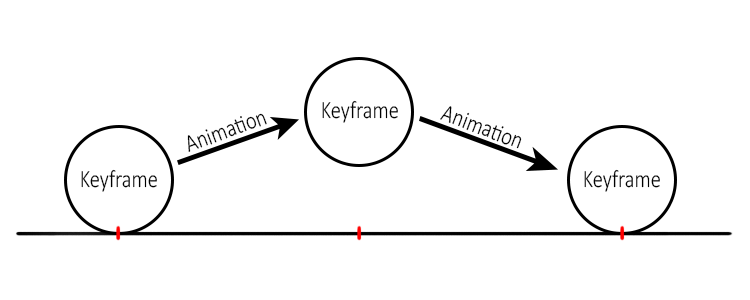
\includegraphics[scale=0.5]{kepek/keyframe_anim.png}
\caption{Kulcsképkocka alapú animáció}
\label{fig:keyframe}
\end{figure}

Ezt a fajta animációt 3D játékfejlesztésben karakter mozgatásához a 2000-es évek elejéig használták, mivel sok memóriát használ, és nem eredményez olyan sima mozgást, mint a csontváz alapú animáció. Ezt a technológiát többek között a Quake 1,2 és 3 alkalmazta.

\subsection{Az md2-es formátum}

1997-ben az idSoftware fejlesztette ki a Quake 2 nevű játékához, kulcsképkocka animáción alapul. Tartalmazza az adott modell geometriáit, és a képkockánkénti animációkat. A fájl adatai olyan struktúrában helyezkednek el, hogy könnyedén kirajzoltatható legyen a GL\_TRIANGLE\_FAN és GL\_TRIANGLE\_STRIP parancsokkal. A formátum két fő részből áll: a fejléc (header) és az adatok (data), viszont nem tartalmazza a modell textúráját. A fejléc egy struktúra, rögön a fájl elején, amely tartalmazza az összes olyan információt a további részről, amelyekre szükség lehet az implementáció során. Ilyen például a textúra szélessége, magassága, egy képkocka mérete, képkockák száma. Az animáláshoz én ezt a módszert választottam, mert viszonylag egyszerű implementálni, a legnagyobb hátránya, a sok memóriahasználat a modern korban már nem olyan nagy probléma, illetve jelen esetben elegendő az animáció részletessége is. 

\section{Csontváz alapú animáció}

A legtöbb mai játék ezt a módszert alkalmazza karakterek mozgatásához. Ez egy olyan hierarchikus mozgás, amelyet nagyon jól lehet használni komplexebb animációkhoz. Ilyen például egy ember, vagy élőlény mozgása. Ember esetén például a kézfej kapcsolatban van az alkarral, az alkar a felkarral, ami pedig a test többi részével. Minden hajlási pont egy új kapcsolódási pontot jelent. Tehát a az ember felkarját megmozdítjuk, mozdul vele a kezének a többi része is. Ez \aref{fig:skeletal} ábrán látható.

% Kép forrása: https://www.openflipper.org/media/plugin_images/skeletalAnimation.png

\begin{figure}[h]
\centering
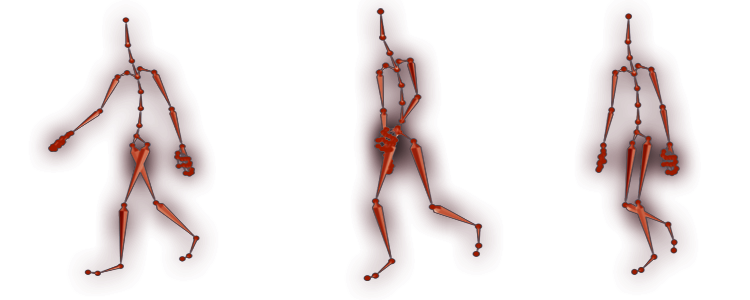
\includegraphics[scale=0.5]{kepek/skeletal_anim.png}
\caption{Testrészek hierarchikus kapcsolódási pontjai emberen}
\label{fig:skeletal}
\end{figure}

De ez nem csak élőlények mozgásának megvalósításához alkalmazható, ilyen például a naprendszer is. Vannak a naprendszerünk bolygói, amelyek a tengelyük, és a központi csillag, a Nap körül is forognak, ha a Nap elmozdul, mozdul vele a teljes naprendszer is, köztük a Föld, és a Hold is. Előnye hogy könnyen létre lehet így hozni dinamikus animációkat, mivel az összes karakter csontjait lehet forgatni, mozgatni, továbbá megkönnyíti a bonyolultabb animációk elkészítését. Hátránya viszont, hogy komplexebbek, így több processzoridőt igényelnek.

\subsection{Csontváz alapú animációhoz tartozó fájlformátum}

Minden, csontváz alapú animáció megvalósításához szükséges fájlformátum két részből áll. Az egyik a modell geometriáit, a másik pedig a csontvázat, kapcsolódási pontokat, eltolást tartalmazza. Ha két csont tartozik minden vertex-hez, a felépítés a következőképp alakul:
\begin{itemize}
\item A vertex x,y,z koordinátája
\item Normálvektor x,y,z iránya
\item Textúra u,v koordinátái
\item Indexek (index1, index2) a csont/eltolás mátrix tömbjéhez (2 csont esetében)
\item Weight1, weight2, ami az egyes csontok átfedési tényezője (2 csont esetében)
\end{itemize}

\section{Interpolációs módszerek}

% Interpoláció: https://hu.wikipedia.org/wiki/Interpol%C3%A1ci%C3%B3#Lagrange-interpol.C3.A1ci.C3.B3

Animációkészítés során többféle interpolációt használhatunk, ami azt jelenti, hogy ismert értékek alapján, a köztes részekre, vagyis nem ismert értékekre adunk közelítést. Többféle interpoláció létezik, amelyek egyikét annak megfelelően használjuk, hogy mit szeretnénk megvalósítani. Korábbi példára visszatérve, például egy redőny leengedéséhez tökéletes a lineáris interpoláció, viszont egy labda pattogás görbéjének megadásához már nem.

\subsection{Lineáris interpoláció}

Ez a legegyszerűbb interpolációs módszer, minden pontot egy egyenessel kötünk össze. Nem összetett mozgásoknál ez megfelelő lehet, viszont ha több mozgás követi egymást rögtön, akkor darabos. Minden előre meghatározott pont, amit érinteni kell egy törést jelent, így komplexebb, sima mozgásokhoz nem alkalmas, ez látható \aref{fig:linear} ábrán.

\begin{figure}[h]
\centering
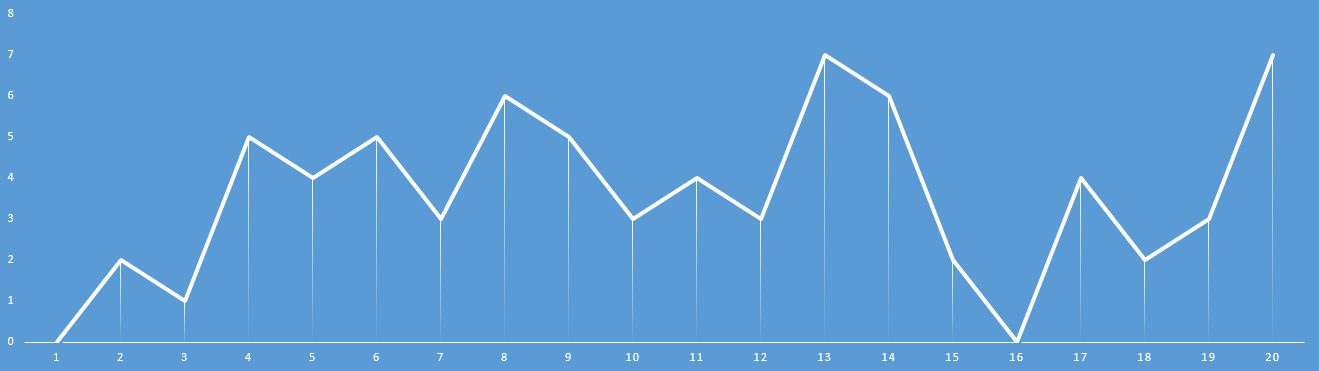
\includegraphics[scale=0.43]{kepek/linear_interpol.png}
\caption{Lineáris interpoláció}
\label{fig:linear}
\end{figure}

\subsection{Lagrange-interpoláció}

Komplexebb animációknál, mint például egy élőlény mozgása, ha nem szeretnénk darabos animációt, ez egy lehetséges megoldás. Mivel a függvény sima, deriváltja folyontos, sokkal életszerűbb megközelítést lehet elérni vele, ez látható \aref{fig:lagrange}-es ábrán. 

\begin{figure}[h]
\centering
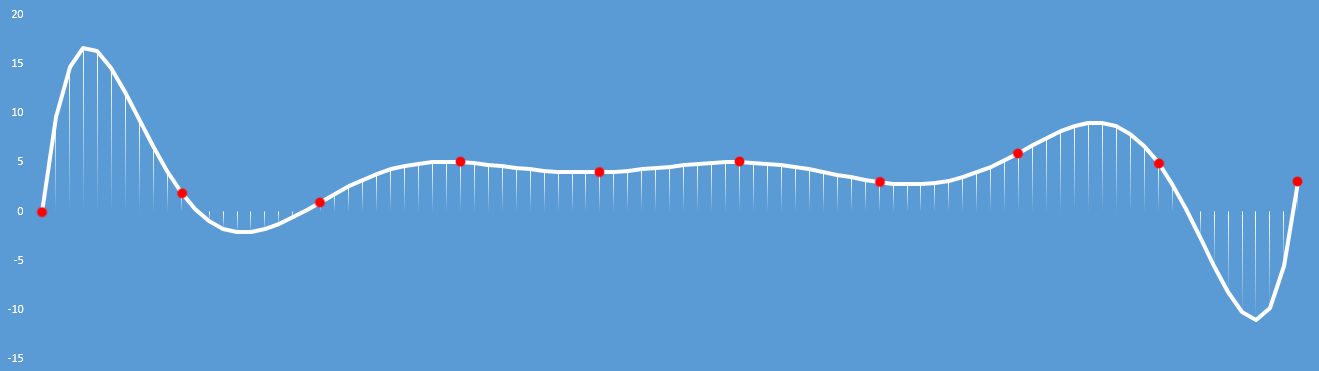
\includegraphics[scale=0.43]{kepek/non_linear_interpol.png}
\caption{Lagrange-interpoláció}
\label{fig:lagrange}
\end{figure}

\subsubsection{Megvalósítás}

A felhasználónak lehetősége van beírni egy x értéket, amelyhez a program kiszámolja az y koordinátát Lagrange-interpolációval. Ez a program azért készült, hogy bemutassa, hogyan működik ez a fajta interpolálás.
Adott két tömb, amelyek tartalmazzák a függvény megadott pontjainak x és y értékeit. A num a tömbök elemeinek számát, az input pedig a bevitt értéket takarja.

\begin{algorithm}[H]
 \KwData{x[]; y[]; num; input; s; t; eredmeny\;}
 \KwResult{Adott x-hez tartozó y koordináta}
\For{i := 0; i < num; i++}{
	s := 1, t := 1\;
	\For{j := 0; j < num; j++}{	
	\If{j != i}{
   		s := s * (input - x[j]);\\
		t := t * (x[i] - x[j])\;
   		}
	}
	eredmeny := eredmeny + ((s / t) * y[i])\;
 }
 \caption{Lagrange-interpoláció implementálása}
\end{algorithm} 

\begin{figure}[h]
\centering
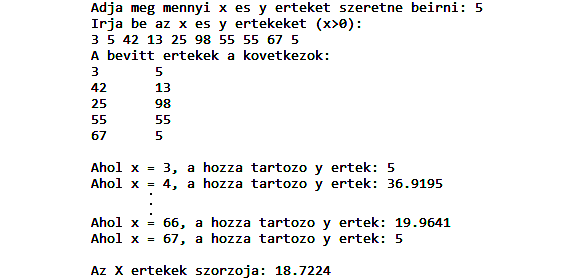
\includegraphics[scale=0.9]{kepek/lagrange_imp.png}
\caption{Lagrange-interpolációs demó}
\label{fig:lagrange_imp}
\end{figure}
